\documentclass[11pt]{article}
\usepackage[utf8]{inputenc}
\usepackage[T1]{fontenc}
\usepackage[margin=2.4cm]{geometry}
\usepackage{booktabs}
\usepackage{amsmath}
\usepackage{graphicx}
\usepackage{float}
\graphicspath{{figures/}}
\setlength{\parskip}{0.5em}
\setlength{\parindent}{0pt}

\title{\vspace{-2.5em}Comparaci\'on de preprocesamientos (Box--Cox, ecualizaci\'on de
histograma y CLAHE) en la segmentaci\'on de grietas con LDA y QDA}
\author{}
\date{}

\begin{document}
\maketitle
\vspace{-3em}

Este informe compara tres t\'ecnicas de \textbf{prefiltrado por contraste} ---
\textbf{Box--Cox}, \textbf{ecualizaci\'on de histograma} (HistEq) y \textbf{CLAHE}
(\emph{Contrast Limited Adaptive Histogram Equalization})--- frente al uso de la
imagen \textbf{sin transformar} (\emph{Raw}), en la segmentaci\'on de grietas a nivel
de p\'ixel con dos clasificadores sensibles a la distribuci\'on: \textbf{LDA} y
\textbf{QDA}. El objetivo es cuantificar c\'omo cada preprocesamiento afecta la
calidad de la segmentaci\'on y el compromiso \emph{precision}--\emph{recall}.

\section*{1. Datos}
Conjunto de grietas de hormig\'on de \"Ozgenel \& Sorgu\c{c}. Cuatro conjuntos de
\textbf{50 im\'agenes} seg\'un la geometr\'ia de la fractura: \textbf{verticales},
\textbf{horizontales}, \textbf{oblicuas} (de izquierda a derecha) y \textbf{grandes}
(la grieta ocupa una porci\'on amplia de la imagen). Cada imagen RGB tiene su
m\'ascara binaria; todas se redimensionan a $256\times256$ y la m\'ascara se
binariza. En total, $4\times50=200$ im\'agenes etiquetadas.

\section*{2. Metodolog\'ia}
\textbf{Preprocesamientos.} Cada imagen se convierte a escala de grises
($0{,}299R+0{,}587G+0{,}114B$) y se obtiene un \'unico canal de intensidad bajo cada
condici\'on:
\begin{itemize}
  \item \textbf{Raw:} intensidad gris cruda normalizada a $[0,1]$ (\emph{baseline}).
  \item \textbf{Box--Cox:} transformaci\'on de Box--Cox con $\lambda$ estimado por
  m\'axima verosimilitud \textbf{por imagen}, seguida de \emph{histogram stretching}
  a $[0,1]$.
  \item \textbf{HistEq:} ecualizaci\'on \emph{global} del histograma
  (\texttt{cv2.equalizeHist}).
  \item \textbf{CLAHE:} ecualizaci\'on adaptativa con l\'imite de contraste
  ($\mathtt{clipLimit}=2{,}0$, mosaico $8\times8$).
\end{itemize}
Las transformaciones son \textbf{por imagen} (cada una con sus propios par\'ametros).

\textbf{Clasificadores.} LDA y QDA a nivel de p\'ixel; la \emph{feature} es la
intensidad del p\'ixel. \textbf{Protocolo por imagen}: para cada imagen se entrena con
una muestra estratificada de hasta $6000$ de sus p\'ixeles (\textbf{los mismos
\'indices en las cuatro condiciones}, de modo que la comparaci\'on es pareada) y se
predice la imagen completa.

\textbf{M\'etricas} (clase grieta): IoU, Dice/F1, \emph{Precision} y \emph{Recall}.
Se reporta \textbf{media\,$\pm$\,desviaci\'on est\'andar sobre las 50 im\'agenes} de
cada conjunto. La \emph{Accuracy} se omite por ser enga\~nosa (la grieta es
$\sim$1\,\% de los p\'ixeles).

\textbf{Significancia.} Cada transformaci\'on se compara \textbf{contra Raw} mediante
un \textbf{test pareado de permutaci\'on} (sign-flip) y el de Wilcoxon, pareando
imagen con imagen, m\'as \textbf{intervalos de confianza al 95\,\% por bootstrap}
(remuestreando \emph{im\'agenes}). Significancia: $^{*}p<0{,}05$, $^{**}p<0{,}01$,
$^{***}p<0{,}001$. En las tablas, \textbf{en negrita} el mejor valor de cada fila.

\section*{3. Resultados}
\begin{table}[H]\centering\small
\caption{Promedio sobre los cuatro conjuntos (200 im\'agenes) de cada m\'etrica, por clasificador y preprocesamiento (\%). En \textbf{negrita} el mejor de cada fila.}\label{tab:avg}
\begin{tabular}{l l cccc}
\toprule
Clasificador & M\'etrica & Raw & Box--Cox & HistEq & CLAHE \\
\midrule
LDA & IoU & \textbf{38.3} & 29.3 & 10.4 & 26.9 \\
 & Dice & \textbf{53.7} & 44.1 & 17.9 & 41.3 \\
 & Precision & \textbf{53.9} & 37.3 & 12.9 & 31.2 \\
 & Recall & 57.3 & 62.9 & 55.4 & \textbf{65.6} \\
\addlinespace
QDA & IoU & \textbf{37.4} & 36.1 & 9.7 & 35.7 \\
 & Dice & \textbf{52.5} & 51.4 & 16.6 & 51.3 \\
 & Precision & \textbf{74.8} & 58.6 & 11.1 & 53.5 \\
 & Recall & 43.7 & 53.4 & \textbf{57.0} & 54.5 \\
\bottomrule
\end{tabular}
\end{table}

\begin{table}[H]\centering\small
\caption{\emph{Intersection over Union} (IoU, \%) de la clase grieta, media\,$\pm$\,desv.\ est.\ sobre las 50 im\'agenes de cada conjunto. Significancia del test pareado de permutaci\'on \emph{frente a Raw}.}\label{tab:iou}
\begin{tabular}{l cccc}
\toprule
M\'etodo & Raw & Box--Cox & HistEq & CLAHE \\
\midrule
\multicolumn{5}{l}{\textit{Verticales} ($\bar\lambda=2.17$)} \\
\quad LDA & \textbf{$41.3\pm16.1$} & $32.9\pm13.6$$^{***}$ & $10.2\pm8.1$$^{***}$ & $29.7\pm14.4$$^{***}$ \\
\quad QDA & \textbf{$39.0\pm17.4$} & $37.6\pm16.5$ & $10.7\pm8.9$$^{***}$ & $38.6\pm14.7$ \\
\addlinespace
\multicolumn{5}{l}{\textit{Horizontales} ($\bar\lambda=1.73$)} \\
\quad LDA & \textbf{$34.9\pm12.9$} & $29.8\pm10.2$$^{***}$ & $10.9\pm12.7$$^{***}$ & $22.9\pm9.0$$^{***}$ \\
\quad QDA & $32.2\pm15.9$ & \textbf{$34.6\pm13.3$$^{*}$} & $9.1\pm11.9$$^{***}$ & $32.1\pm12.9$ \\
\addlinespace
\multicolumn{5}{l}{\textit{Oblicuas (izq.\,$\to$\,der.)} ($\bar\lambda=2.11$)} \\
\quad LDA & \textbf{$40.7\pm17.1$} & $29.5\pm12.0$$^{***}$ & $10.3\pm7.8$$^{***}$ & $29.2\pm10.8$$^{***}$ \\
\quad QDA & \textbf{$41.0\pm16.3$} & $39.0\pm13.2$ & $8.2\pm6.8$$^{***}$ & $38.6\pm11.5$ \\
\addlinespace
\multicolumn{5}{l}{\textit{Grandes} ($\bar\lambda=2.38$)} \\
\quad LDA & \textbf{$36.2\pm11.9$} & $25.0\pm8.9$$^{***}$ & $10.3\pm3.9$$^{***}$ & $25.9\pm8.5$$^{***}$ \\
\quad QDA & \textbf{$37.6\pm10.8$} & $33.1\pm11.2$$^{***}$ & $10.7\pm5.2$$^{***}$ & $33.3\pm9.2$$^{***}$ \\
\bottomrule
\end{tabular}
\end{table}

\begin{table}[H]\centering\small
\caption{Coeficiente Dice/F1 (\%) de la clase grieta, media\,$\pm$\,desv.\ est. Significancia frente a Raw.}\label{tab:dice}
\begin{tabular}{l cccc}
\toprule
M\'etodo & Raw & Box--Cox & HistEq & CLAHE \\
\midrule
\multicolumn{5}{l}{\textit{Verticales} ($\bar\lambda=2.17$)} \\
\quad LDA & \textbf{$56.6\pm17.2$} & $48.0\pm16.1$$^{***}$ & $17.6\pm13.1$$^{***}$ & $44.1\pm15.8$$^{***}$ \\
\quad QDA & $53.7\pm19.6$ & $52.4\pm19.0$ & $18.2\pm13.7$$^{***}$ & \textbf{$54.0\pm16.5$} \\
\addlinespace
\multicolumn{5}{l}{\textit{Horizontales} ($\bar\lambda=1.73$)} \\
\quad LDA & \textbf{$50.4\pm14.4$} & $45.0\pm11.9$$^{***}$ & $17.5\pm18.8$$^{***}$ & $36.4\pm11.6$$^{***}$ \\
\quad QDA & $46.4\pm20.2$ & \textbf{$49.9\pm16.2$$^{*}$} & $14.9\pm17.4$$^{***}$ & $47.1\pm16.0$ \\
\addlinespace
\multicolumn{5}{l}{\textit{Oblicuas (izq.\,$\to$\,der.)} ($\bar\lambda=2.11$)} \\
\quad LDA & \textbf{$55.7\pm18.5$} & $44.2\pm14.4$$^{***}$ & $17.8\pm12.2$$^{***}$ & $44.2\pm12.8$$^{***}$ \\
\quad QDA & \textbf{$56.1\pm18.2$} & $54.8\pm14.3$ & $14.5\pm11.1$$^{***}$ & $54.7\pm12.6$ \\
\addlinespace
\multicolumn{5}{l}{\textit{Grandes} ($\bar\lambda=2.38$)} \\
\quad LDA & \textbf{$52.1\pm13.2$} & $39.2\pm11.2$$^{***}$ & $18.5\pm6.4$$^{***}$ & $40.4\pm10.4$$^{***}$ \\
\quad QDA & \textbf{$53.7\pm11.6$} & $48.7\pm12.8$$^{***}$ & $19.0\pm8.1$$^{***}$ & $49.3\pm10.4$$^{***}$ \\
\bottomrule
\end{tabular}
\end{table}

\begin{table}[H]\centering\small
\caption{\emph{Precision} (\%) de la clase grieta, media\,$\pm$\,desv.\ est. Significancia frente a Raw.}\label{tab:prec}
\begin{tabular}{l cccc}
\toprule
M\'etodo & Raw & Box--Cox & HistEq & CLAHE \\
\midrule
\multicolumn{5}{l}{\textit{Verticales} ($\bar\lambda=2.17$)} \\
\quad LDA & \textbf{$58.2\pm21.1$} & $42.6\pm19.7$$^{***}$ & $11.4\pm11.1$$^{***}$ & $34.3\pm16.4$$^{***}$ \\
\quad QDA & \textbf{$74.6\pm21.8$} & $61.3\pm23.4$$^{***}$ & $11.7\pm10.9$$^{***}$ & $57.5\pm18.8$$^{***}$ \\
\addlinespace
\multicolumn{5}{l}{\textit{Horizontales} ($\bar\lambda=1.73$)} \\
\quad LDA & \textbf{$48.5\pm17.4$} & $39.3\pm14.1$$^{***}$ & $15.9\pm23.1$$^{***}$ & $26.2\pm10.1$$^{***}$ \\
\quad QDA & \textbf{$77.8\pm10.6$} & $63.5\pm17.3$$^{***}$ & $10.8\pm16.6$$^{***}$ & $54.0\pm14.2$$^{***}$ \\
\addlinespace
\multicolumn{5}{l}{\textit{Oblicuas (izq.\,$\to$\,der.)} ($\bar\lambda=2.11$)} \\
\quad LDA & \textbf{$56.6\pm24.4$} & $36.5\pm17.0$$^{***}$ & $13.4\pm16.5$$^{***}$ & $33.6\pm12.6$$^{***}$ \\
\quad QDA & \textbf{$78.8\pm19.9$} & $61.3\pm19.8$$^{***}$ & $10.0\pm13.6$$^{***}$ & $55.8\pm14.8$$^{***}$ \\
\addlinespace
\multicolumn{5}{l}{\textit{Grandes} ($\bar\lambda=2.38$)} \\
\quad LDA & \textbf{$52.4\pm18.9$} & $30.6\pm14.3$$^{***}$ & $10.8\pm4.1$$^{***}$ & $30.7\pm10.6$$^{***}$ \\
\quad QDA & \textbf{$67.9\pm17.0$} & $48.1\pm19.1$$^{***}$ & $12.0\pm10.7$$^{***}$ & $46.7\pm14.5$$^{***}$ \\
\bottomrule
\end{tabular}
\end{table}

\begin{table}[H]\centering\small
\caption{\emph{Recall} (\%) de la clase grieta, media\,$\pm$\,desv.\ est. Significancia frente a Raw.}\label{tab:rec}
\begin{tabular}{l cccc}
\toprule
M\'etodo & Raw & Box--Cox & HistEq & CLAHE \\
\midrule
\multicolumn{5}{l}{\textit{Verticales} ($\bar\lambda=2.17$)} \\
\quad LDA & $59.0\pm12.9$ & $64.5\pm16.1$$^{***}$ & $55.2\pm36.7$ & \textbf{$67.5\pm12.4$$^{***}$} \\
\quad QDA & $45.6\pm19.1$ & $53.7\pm21.5$$^{***}$ & \textbf{$61.6\pm34.5$$^{***}$} & $56.3\pm18.2$$^{***}$ \\
\addlinespace
\multicolumn{5}{l}{\textit{Horizontales} ($\bar\lambda=1.73$)} \\
\quad LDA & $54.7\pm11.7$ & $57.6\pm14.6$$^{***}$ & $38.2\pm36.8$$^{***}$ & \textbf{$63.6\pm11.8$$^{***}$} \\
\quad QDA & $37.0\pm19.6$ & $46.4\pm19.8$$^{***}$ & $40.2\pm38.5$ & \textbf{$48.4\pm20.1$$^{***}$} \\
\addlinespace
\multicolumn{5}{l}{\textit{Oblicuas (izq.\,$\to$\,der.)} ($\bar\lambda=2.11$)} \\
\quad LDA & $59.1\pm11.1$ & $64.2\pm14.2$$^{***}$ & $57.1\pm34.2$ & \textbf{$68.3\pm10.6$$^{***}$} \\
\quad QDA & $45.9\pm17.2$ & $55.5\pm17.6$$^{***}$ & $55.5\pm37.1$$^{**}$ & \textbf{$57.5\pm15.8$$^{***}$} \\
\addlinespace
\multicolumn{5}{l}{\textit{Grandes} ($\bar\lambda=2.38$)} \\
\quad LDA & $56.3\pm8.3$ & $65.2\pm11.0$$^{***}$ & \textbf{$71.2\pm20.7$$^{***}$} & $63.1\pm8.0$$^{***}$ \\
\quad QDA & $46.4\pm10.7$ & $58.2\pm13.5$$^{***}$ & \textbf{$70.9\pm21.5$$^{***}$} & $56.0\pm10.6$$^{***}$ \\
\bottomrule
\end{tabular}
\end{table}

\medskip
\textbf{Comparaci\'on directa entre transformaciones.} Las tablas anteriores comparan
cada preprocesamiento contra \emph{Raw}. Las dos siguientes contrastan las
transformaciones \textbf{entre s\'i} (pareando imagen con imagen), que es la
comparaci\'on relevante para decidir entre ellas.

\begin{table}[H]\centering\small
\caption{Comparaci\'on directa \textbf{Box--Cox vs HistEq}: $\Delta=$ media(Box--Cox)$-$media(HistEq) en puntos porcentuales, pareada imagen con imagen (positivo $\Rightarrow$ Box--Cox mejor). Significancia del test de permutaci\'on.}\label{tab:bc_he}
\begin{tabular}{l cccc}
\toprule
M\'etodo & IoU & Dice & Precision & Recall \\
\midrule
\multicolumn{5}{l}{\textit{Verticales}} \\
\quad LDA & $+22.7$$^{***}$ & $+30.4$$^{***}$ & $+31.2$$^{***}$ & $+9.3$$^{*}$ \\
\quad QDA & $+26.9$$^{***}$ & $+34.2$$^{***}$ & $+49.7$$^{***}$ & $-7.9$ \\
\addlinespace
\multicolumn{5}{l}{\textit{Horizontales}} \\
\quad LDA & $+18.9$$^{***}$ & $+27.5$$^{***}$ & $+23.5$$^{***}$ & $+19.4$$^{***}$ \\
\quad QDA & $+25.5$$^{***}$ & $+35.0$$^{***}$ & $+52.7$$^{***}$ & $+6.2$ \\
\addlinespace
\multicolumn{5}{l}{\textit{Oblicuas (izq.\,$\to$\,der.)}} \\
\quad LDA & $+19.2$$^{***}$ & $+26.4$$^{***}$ & $+23.1$$^{***}$ & $+7.1$$^{*}$ \\
\quad QDA & $+30.8$$^{***}$ & $+40.3$$^{***}$ & $+51.3$$^{***}$ & $+0.0$ \\
\addlinespace
\multicolumn{5}{l}{\textit{Grandes}} \\
\quad LDA & $+14.6$$^{***}$ & $+20.7$$^{***}$ & $+19.8$$^{***}$ & $-6.0$$^{**}$ \\
\quad QDA & $+22.4$$^{***}$ & $+29.7$$^{***}$ & $+36.0$$^{***}$ & $-12.8$$^{***}$ \\
\bottomrule
\end{tabular}
\end{table}

\begin{table}[H]\centering\small
\caption{Comparaci\'on directa \textbf{Box--Cox vs CLAHE}: $\Delta=$ media(Box--Cox)$-$media(CLAHE) en puntos porcentuales, pareada imagen con imagen (positivo $\Rightarrow$ Box--Cox mejor). Significancia del test de permutaci\'on.}\label{tab:bc_cl}
\begin{tabular}{l cccc}
\toprule
M\'etodo & IoU & Dice & Precision & Recall \\
\midrule
\multicolumn{5}{l}{\textit{Verticales}} \\
\quad LDA & $+3.2$$^{*}$ & $+3.8$$^{*}$ & $+8.3$$^{**}$ & $-2.9$$^{**}$ \\
\quad QDA & $-1.0$ & $-1.6$ & $+3.8$ & $-2.6$ \\
\addlinespace
\multicolumn{5}{l}{\textit{Horizontales}} \\
\quad LDA & $+6.9$$^{***}$ & $+8.6$$^{***}$ & $+13.2$$^{***}$ & $-5.9$$^{***}$ \\
\quad QDA & $+2.5$$^{***}$ & $+2.7$$^{***}$ & $+9.5$$^{***}$ & $-2.0$$^{*}$ \\
\addlinespace
\multicolumn{5}{l}{\textit{Oblicuas (izq.\,$\to$\,der.)}} \\
\quad LDA & $+0.3$ & $+0.0$ & $+2.9$ & $-4.1$$^{***}$ \\
\quad QDA & $+0.3$ & $+0.0$ & $+5.5$$^{*}$ & $-2.0$$^{*}$ \\
\addlinespace
\multicolumn{5}{l}{\textit{Grandes}} \\
\quad LDA & $-0.9$ & $-1.3$ & $-0.1$ & $+2.1$ \\
\quad QDA & $-0.2$ & $-0.6$ & $+1.4$ & $+2.2$ \\
\bottomrule
\end{tabular}
\end{table}

\textbf{Box--Cox supera a HistEq} de forma masiva y significativa en IoU, Dice y
\emph{precision} en los ocho casos (entre $+15$ y $+53$ puntos, $p<0{,}001$), lo que
confirma que HistEq es el preprocesamiento m\'as d\'ebil; HistEq solo iguala o supera
en \emph{recall} de manera inconsistente. \textbf{Frente a CLAHE} las diferencias son
mucho menores: Box--Cox tiende a mayor \emph{precision} (y a mayor IoU/Dice en grietas
horizontales), mientras que CLAHE consigue mayor \emph{recall}; en IoU/Dice ambos
resultan \textbf{estad\'isticamente equivalentes} en la mayor\'ia de los conjuntos
(diferencias peque\~nas y no significativas, salvo en horizontales, donde gana
Box--Cox).

\section*{4. Lectura de los resultados}
El conteo de ``mejor por fila'' sobre las 32 combinaciones (4 conjuntos $\times$ 2
clasificadores $\times$ 4 m\'etricas) es: \textbf{Raw 21},
CLAHE 6, HistEq 3 y Box--Cox
2. Las conclusiones principales:
\begin{itemize}
  \item \textbf{Ninguna transformaci\'on mejora la calidad global de forma
  consistente.} \emph{Raw} es el mejor en IoU, Dice y \emph{precision} en casi todos
  los casos. Las tres t\'ecnicas siguen el patr\'on cl\'asico: \textbf{suben el
  \emph{recall} a costa de la \emph{precision}}.
  \item \textbf{HistEq es, con diferencia, la peor.} La ecualizaci\'on global
  destruye IoU, Dice y \emph{precision} (la \emph{precision} cae a $\sim$10--13\,\%,
  todas con $p<0{,}001$) y es \textbf{muy inestable}: la desviaci\'on del \emph{recall}
  entre im\'agenes ronda el 35\,\% (frente a 11--19\,\% en las dem\'as), porque satura
  el contraste y a menudo etiqueta como grieta gran parte del fondo.
  \item \textbf{CLAHE y Box--Cox son comparables y mucho m\'as suaves.} CLAHE entrega
  el \emph{recall} m\'as alto y estable (mejor detecci\'on); Box--Cox conserva algo
  mejor la \emph{precision}. Ambas son el preprocesamiento de elecci\'on si la
  prioridad es \textbf{no pasar por alto la fractura}. No obstante, el promedio oculta
  variabilidad por imagen: \textbf{en algunos casos Box--Cox supera claramente a CLAHE}
  en calidad (IoU/Dice), recuperando mejor la red completa de la grieta
  (v\'ease la Figura~\ref{fig:bcwin}).
  \item \textbf{El clasificador importa.} En \textbf{QDA}, CLAHE y Box--Cox apenas
  alteran IoU/Dice (cambios peque\~nos, a menudo no significativos): son ``seguras''
  para ganar \emph{recall} sin sacrificar calidad. En \textbf{LDA}, en cambio, todas
  las transformaciones reducen IoU/Dice de forma significativa.
  \item \textbf{\'Unico caso favorable en calidad:} QDA con Box--Cox en grietas
  \emph{horizontales} (IoU $+2{,}4$, Dice $+3{,}5$; $p<0{,}05$), donde el aumento de
  \emph{recall} compensa la p\'erdida de \emph{precision}.
\end{itemize}

\section*{5. Ejemplos}
Un ejemplo por tipo de grieta (clasificador QDA). De izquierda a derecha: imagen RGB,
m\'ascara real y segmentaci\'on bajo Raw, Box--Cox, HistEq y CLAHE. Se aprecia c\'omo
HistEq \textbf{inunda} la predicci\'on de falsos positivos (\emph{recall} alto pero
\emph{precision} muy baja), mientras CLAHE y Box--Cox engrosan moderadamente la grieta
respecto de Raw. La \'ultima figura (con t\'itulos en IoU/Dice) muestra un caso en que
\textbf{Box--Cox supera claramente a CLAHE} en calidad, recordando que el promedio
oculta variabilidad por imagen.

\begin{figure}[H]\centering
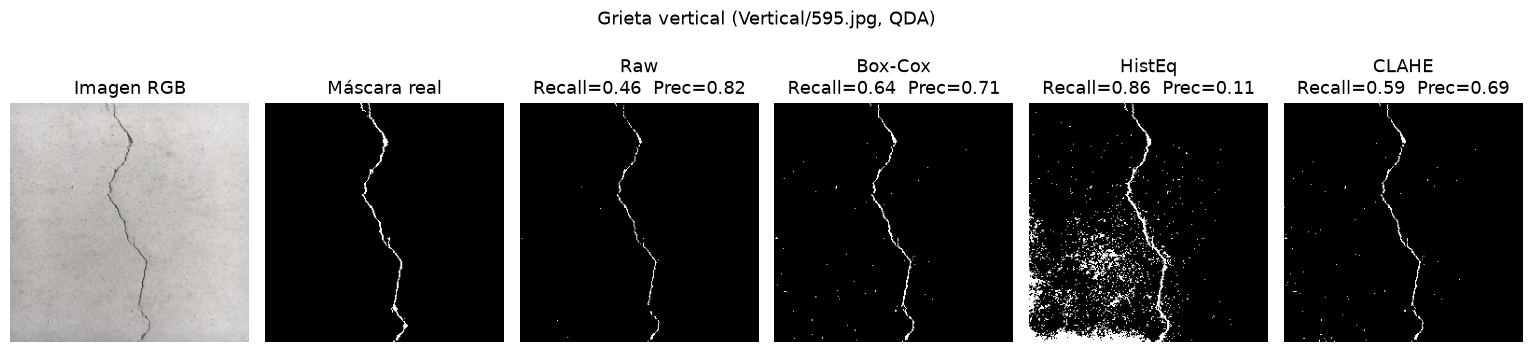
\includegraphics[width=\linewidth]{preproc_Vertical.png}
\caption{Grieta vertical.}
\end{figure}

\begin{figure}[H]\centering
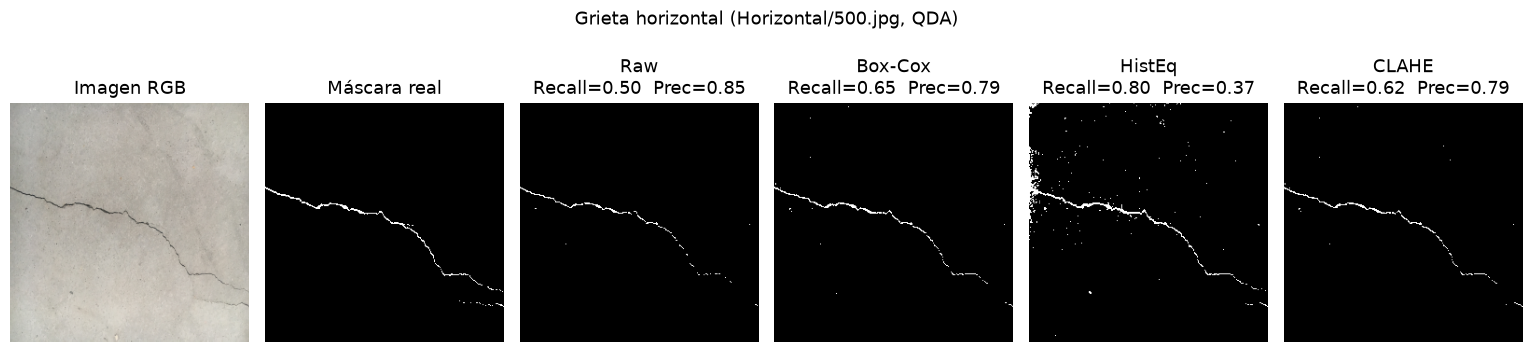
\includegraphics[width=\linewidth]{preproc_Horizontal.png}
\caption{Grieta horizontal.}
\end{figure}

\begin{figure}[H]\centering
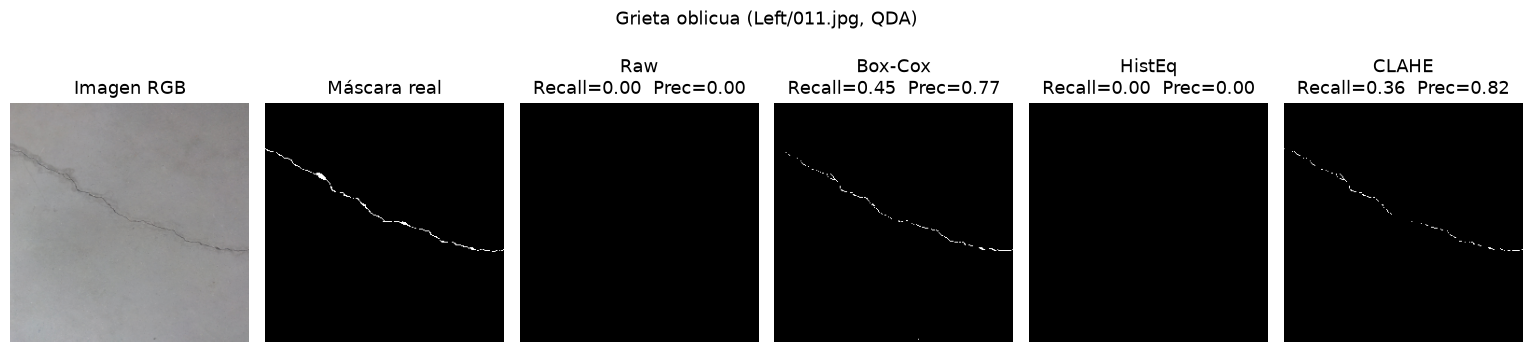
\includegraphics[width=\linewidth]{preproc_Left.png}
\caption{Grieta oblicua.}
\end{figure}

\begin{figure}[H]\centering
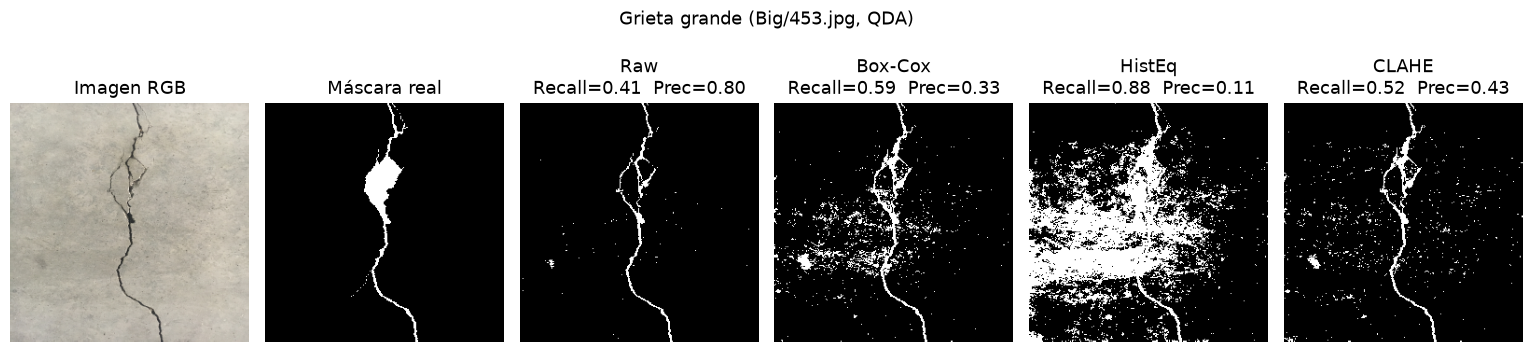
\includegraphics[width=\linewidth]{preproc_Big.png}
\caption{Grieta grande: HistEq satura la imagen de falsos positivos.}
\end{figure}

\begin{figure}[H]\centering
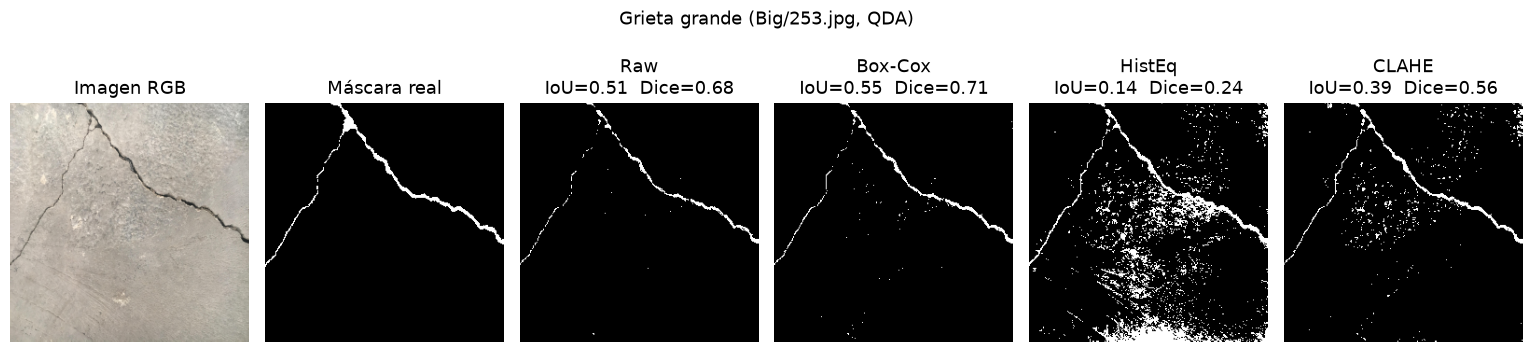
\includegraphics[width=\linewidth]{preproc_BoxCoxWin.png}
\caption{Caso favorable a Box--Cox frente a CLAHE (grieta grande, QDA; t\'itulos en
IoU/Dice). Box--Cox recupera la red completa de la grieta y \textbf{supera tanto a
CLAHE como a Raw} en calidad, mientras CLAHE queda m\'as fragmentada y ruidosa. Ilustra
que, pese a su comportamiento medio similar, ambos preprocesamientos no son
intercambiables imagen a imagen.}\label{fig:bcwin}
\end{figure}

\section*{6. Conclusi\'on}
Sobre 200 im\'agenes con medidas de incertidumbre y tests pareados, \textbf{ninguno de
los tres prefiltrados mejora la calidad global de la segmentaci\'on respecto de usar la
imagen sin transformar}; todos intercambian \emph{precision} por \emph{recall}. La
\textbf{ecualizaci\'on global de histograma (HistEq) es claramente perjudicial} y debe
descartarse. \textbf{CLAHE} y \textbf{Box--Cox} son alternativas suaves y de efecto
similar: \'utiles cuando la prioridad es \textbf{maximizar la detecci\'on}
(\emph{recall}), especialmente con \textbf{QDA}, donde no degradan apreciablemente
IoU/Dice. Si la prioridad es una delimitaci\'on fina de la grieta (mayor IoU/Dice),
conviene usar la imagen \textbf{Raw} o combinar CLAHE/Box--Cox con un
post-procesamiento que recupere \emph{precision}.

\end{document}
